%\documentclass[10pt,notes]{beamer}       % print frame + notes
%\documentclass[10pt, notes=only]{beamer}   % only notes
\documentclass[11pt]{beamer}              % only frames

%%%%%% IF YOU WOULD LIKE TO CREATE LECTURE NOTES COMMENT OUT THE FOlLOWING TWO LINES
%\usepackage{pgfpages}
%\setbeameroption{show notes on second screen=bottom} % Both

\usepackage{graphicx}
\DeclareGraphicsExtensions{.pdf,.png,.jpg}
\usepackage{color}
\usetheme{winslab}
\usepackage[utf8]{inputenc}
\usepackage[english]{babel}
\usepackage{amsmath}
\usepackage{amsfonts}
\usepackage{amssymb}




\usepackage{algorithm2e,algorithmicx,algpseudocode}
\algnewcommand\Input{\item[\textbf{Input:}]}%
\algnewcommand\Output{\item[\textbf{Output:}]}%
\newcommand\tab[1][1cm]{\hspace*{#1}}

\algnewcommand{\Implement}[2]{\item[\textbf{Implements:}] #1 \textbf{Instance}: #2}%
\algnewcommand{\Use}[2]{\item[\textbf{Uses:}] #1 \textbf{Instance}: #2}%
\algnewcommand{\Trigger}[1]{\Statex{\textbf{Trigger:} (#1)}}%
\algnewcommand{\Events}[1]{\item[\textbf{Events:}] #1}%
\algnewcommand{\Need}[1]{\item[\textbf{Needs:}] #1}%
\algnewcommand{\Event}[2]{\Statex\item[\textbf{On#1:}](#2) \textbf{do}}%
\algnewcommand{\Trig}[3]{\State \textbf{Trigger}  #1.#2 (#3) }%
\def\true{\textbf{T}}
\def\false{\textbf{F}}


\author[HUSEYIN SAGIRKAYA]{HUSEYIN SAGIRKAYA\\\href{mailto:huseyin.sagirkaya@metu.edu.tr}{huseyin.sagirkaya@metu.edu.tr}}
%\author[H.\,Sagirkaya]
%{%
%  \texorpdfstring{
%    \begin{columns}%[onlytextwidth]
%      \column{.45\linewidth}
%      \centering
%      Huseyin Sagirkaya\\
%      \href{mailto:huseyin.sagirkaya@metu.edu.tr}{huseyin.sagirkaya@metu.edu.tr}
%      \column{.45\linewidth}
%      \centering
%      Huseyin Sagirkaya\\
%      \href{mailto:huseyin.sagirkaya@metu.edu.tr}{huseyin.sagirkaya@metu.edu.tr}
%    \end{columns}
%  }
%  {Huseyin Sagirkaya}
%}

\title[WINS Beamer Template]{WINS Lab Beamer Presentation Template}
\subtitle[Distributed Computing Algorithms]{Dolev-Klawe-Rodeh and Echo with Extinction Leader Election Algorithms}
%\date{13/05/2024} 

\begin{document}

\begin{frame}[plain]
\titlepage
\note{In this talk, I will present .... Please answer the following questions:
\begin{enumerate}
\item Why are you giving presentation?
\item What is your desired outcome?
\item What does the audience already know  about your topic?
\item What are their interests?
\item What are key points?
\end{enumerate}
}
\end{frame}


\begin{frame}
    \frametitle{Outline of the Presentation}
   
\begin{enumerate}

\item Outline 
\item Problem and background
\item Design and methods
\item Major findings
\item Conclusion and recommendations 
\end{enumerate} 

\end{frame}



%
%\part{This the First Part of the Presentation}
%\begin{frame}
%        \partpage
%\end{frame}
%

%\begin{frame}
%        \sectionpage
%\end{frame}

\begin{frame}{The problem}
\framesubtitle{In an election algorithm, each computation should terminate in a configuration where one process is the leader.}

\begin{block}{The Problem Name} 
Selection a leader ensures continuous coordination between entities. These algorithms also provide a means to recover from failures of the coordinator.
Define leader in a directed ring and undirected networks. 
\end{block}
Distributed system is a collection of independent processes that communicate with each other and cooperate achieving a common goal.

\note{}
\end{frame}


\begin{frame}
\frametitle{Dolev-Klawe-Rodeh and Echo with Extinction Leader Election Algorithms}
\framesubtitle{}
This presentation presents the detailed explanation of the leader selection algorithms;
\item Choosing the leader in a circular ring, where processors choose a single leader with the greatest ID at the end of the Dolev-Klawe-Rodeh algorithm.
\item Choosing the leader in undirected network working for any topology, Echo Algorithm with Extinction.
\begin{itemize}
\item Determinaton of the algorithms time complexity and message complexity.
\item Outputs of the algorithms.
\item Conclusion and trade-offs.
\end{itemize}

\end{frame}



\begin{frame}
\frametitle{Motivation/Importance}
\framesubtitle{}
\item The leader has the responsibility of system management. 
\item For example the client-server model of resource management: 
\item The server is the a leader. Client processes send requests for resources to the server
\item A centralized database manager maintaining a queue of pending read and writes and processes offering a simple solution with manageable complexity.
\item When the leader (i.e., coordinator) fails, a new leader is needed to be elected. Selection a leader ensures continuous coordination between processes.
\end{frame}



\frame{
\item Various election algorithms have been proposed for the leader election. Bully Algorithm has been presented by Gracia- Molina in 1982. 
But its disadvantage is it requires that every process should know the identity of every other process. So it increases traffic. 
\item There are also various ring election algorithms. 
\item The Chang-Robert algorithm targets a directed ring. The idea is that only the message with highset ID completes the trip.
\item Franklins case, message in uses an bidirectional ring to improve for complexity. 
\item Dolew Klawe Rodeh algorithm changes the Franklins algorithm to unidirectional ring meaning a message cannot travel in both direction. 
\item Echo algorithm with extinction can work for any topology. The Echo Algorithm facilitates the selection of a leader orcoordinator among the processes in a distributed system.
}


\begin{frame}{Dolev-Klawe-Rodeh algorithm}
\item  The Dolev-Klawe-Rodeh algorithm uses directed rings which messages cannot travel in both directions. 
\item Active process whose ID is p and next active neighbors are q and r. 
\item The Ids are collected at r. There are three cases to evaluate the election process.
If \[ p > q \] and r; r remains active and progress to the next election round
If \[ p < q \] or r; r becomes passive
If p=q and r; r becomes the leader. 
\begin{figure}
    \centering
    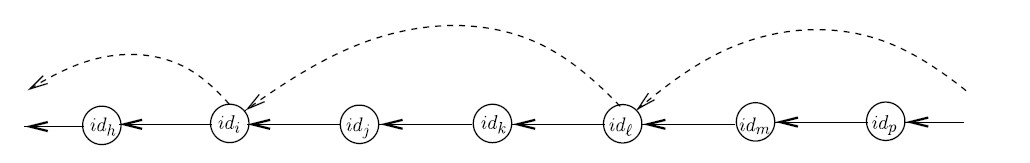
\includegraphics[scale=0.3]{figures/Screen2.jpg}
    \caption{Ring topology}
    \label{fig:Ring topology}
\end{figure}
\end{frame}

\begin{frame}{Echo algorithm with extinction algorithm}
\item Propagate an "echo" message through the network. 
Echo messages are forwarded among processes, so every process knows others' status or candidacy. 
Processes that haven't heard from any higher-priority process declare themselves as leaders and broadcast victory messages.
When a process p in a wave q is hit by a wave r.
If \[ q < r \] then p makes the sender its parent, switches to the wave r.
If \[ q > r \] then p continues with the wave tagged with q.
If q=r then p treats the incoming message according to the echo algorithm of the wave q.
If the wave tagged with p completes by executing a decide event at p, then p becomes the leader.
\begin{figure}
    \centering
    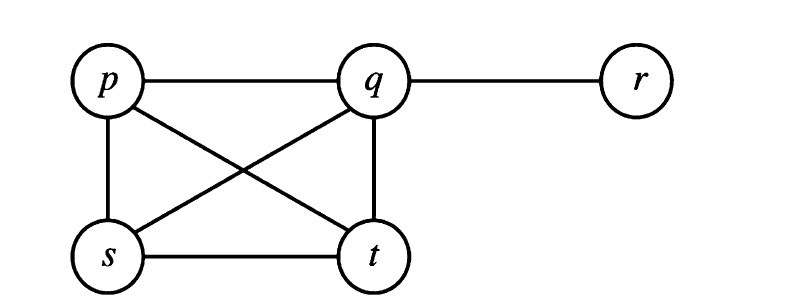
\includegraphics[scale=0.25]{figures/Screen3.jpg}
    \caption{Ring topology}
    \label{fig:Ring topology}
\end{figure}
\end{frame}




\begin{frame}{}
\framesubtitle{Major Results}

\begin{figure}
    \centering
    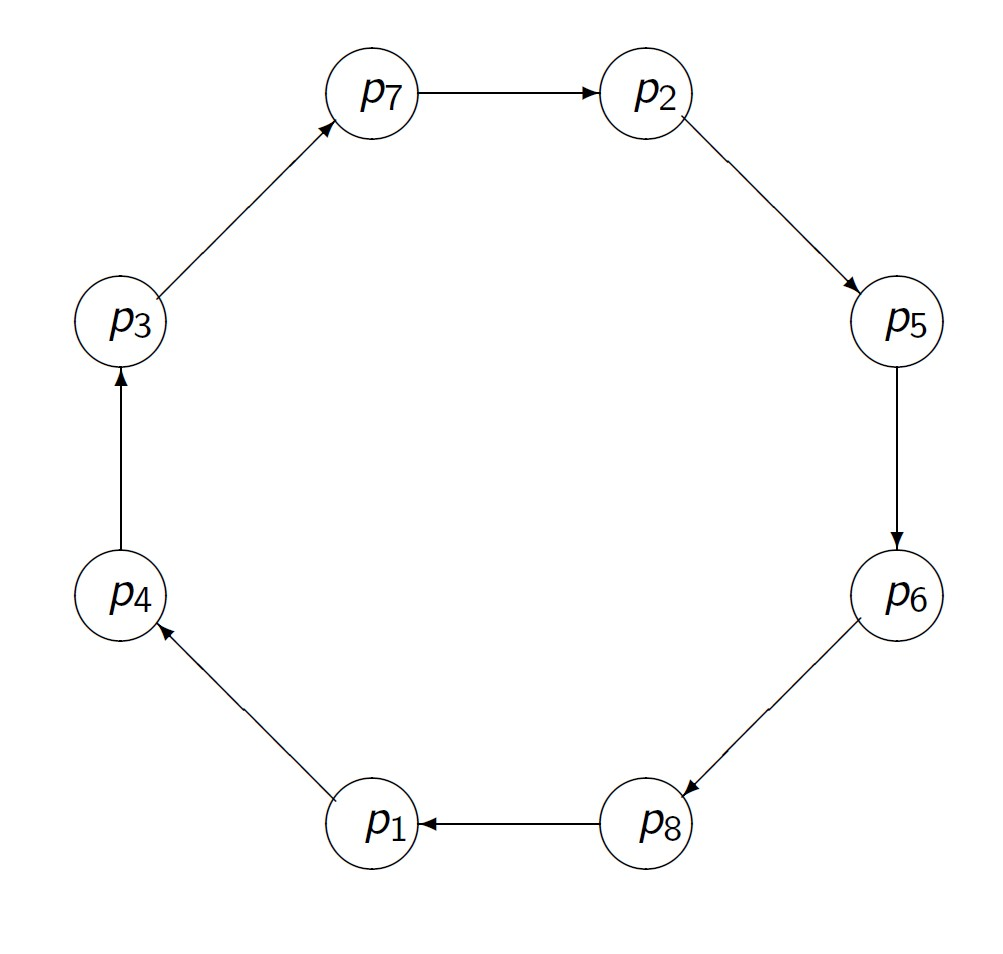
\includegraphics[scale=0.3]{figures/Screen7.jpg}
    \caption{Ring topology}
    \label{fig:Ring topology}
\end{figure}
\note{
}
\end{frame}


\begin{frame}{}
\framesubtitle{Major Results}

\begin{figure}
    \centering
    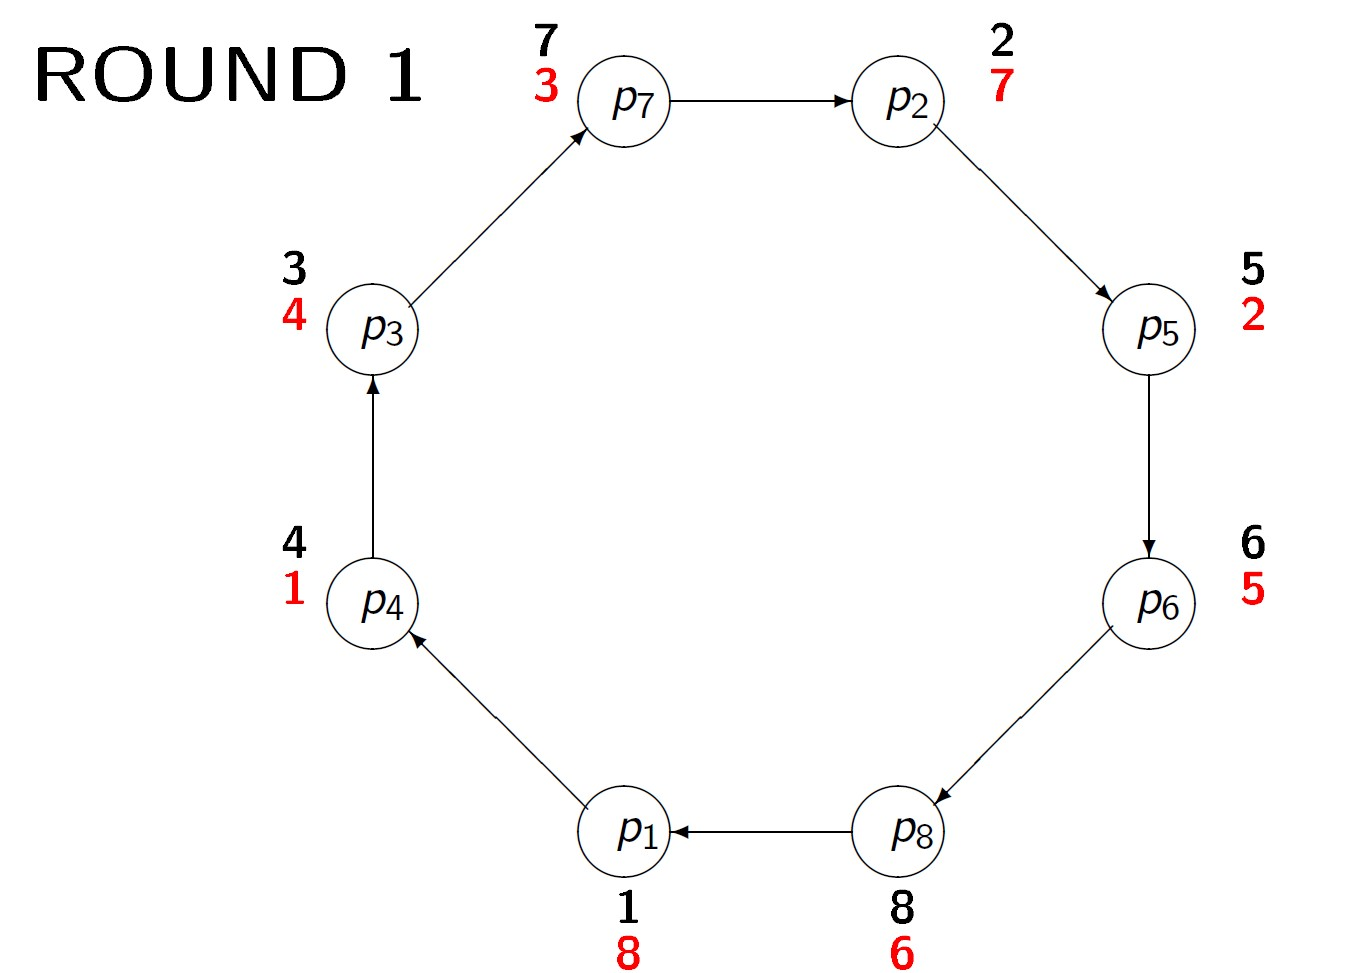
\includegraphics[scale=0.3]{figures/Screen9.jpg}
    \caption{Ring topology}
    \label{fig:Ring topology}
\end{figure}
\note{
}
\end{frame}


\begin{frame}{}
\framesubtitle{Major Results}

\begin{figure}
    \centering
    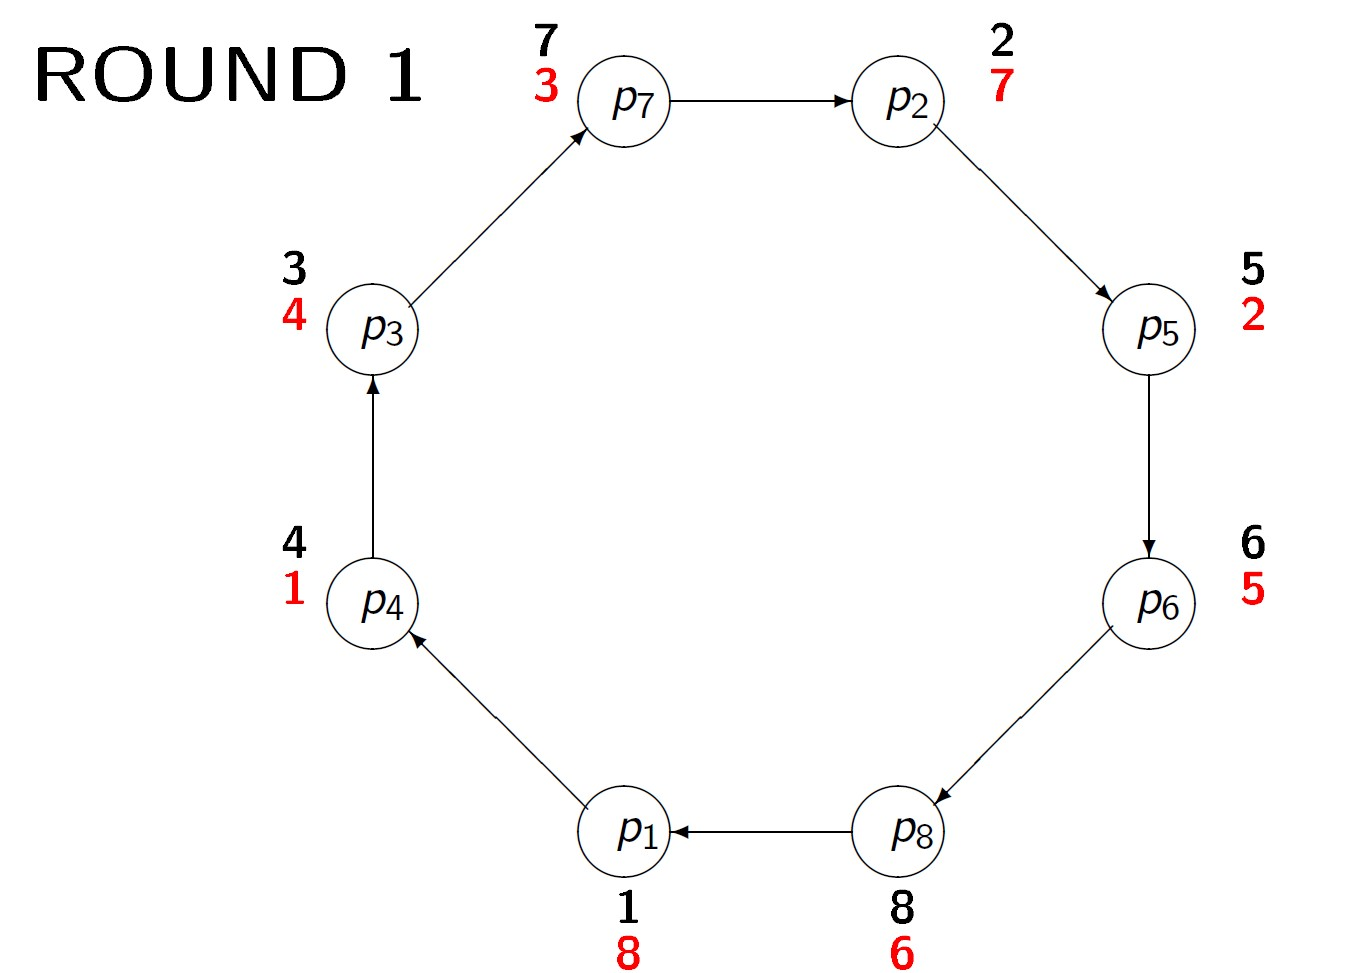
\includegraphics[scale=0.3]{figures/Screen9.jpg}
    \caption{Ring topology}
    \label{fig:Ring topology}
\end{figure}
\note{
}
\end{frame}



\begin{frame}{}
\framesubtitle{Major Results}

\begin{figure}
    \centering
    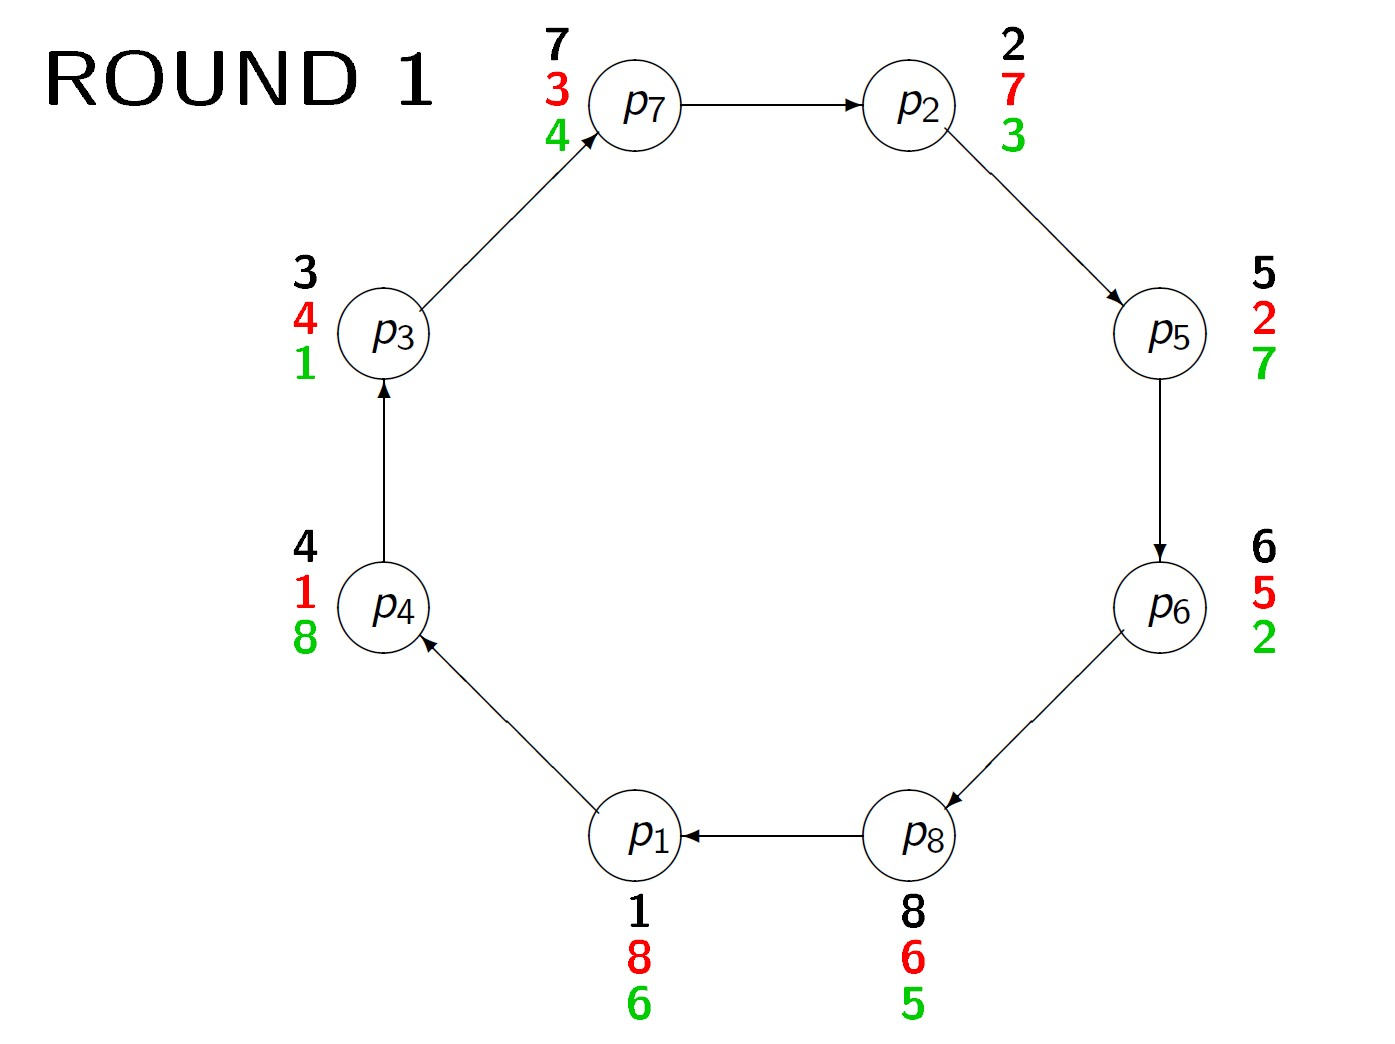
\includegraphics[scale=0.3]{figures/Screen10.jpg}
    \caption{Ring topology}
    \label{fig:Ring topology}
\end{figure}
\note{
}
\end{frame}


\begin{frame}{}
\framesubtitle{Major Results}

\begin{figure}
    \centering
    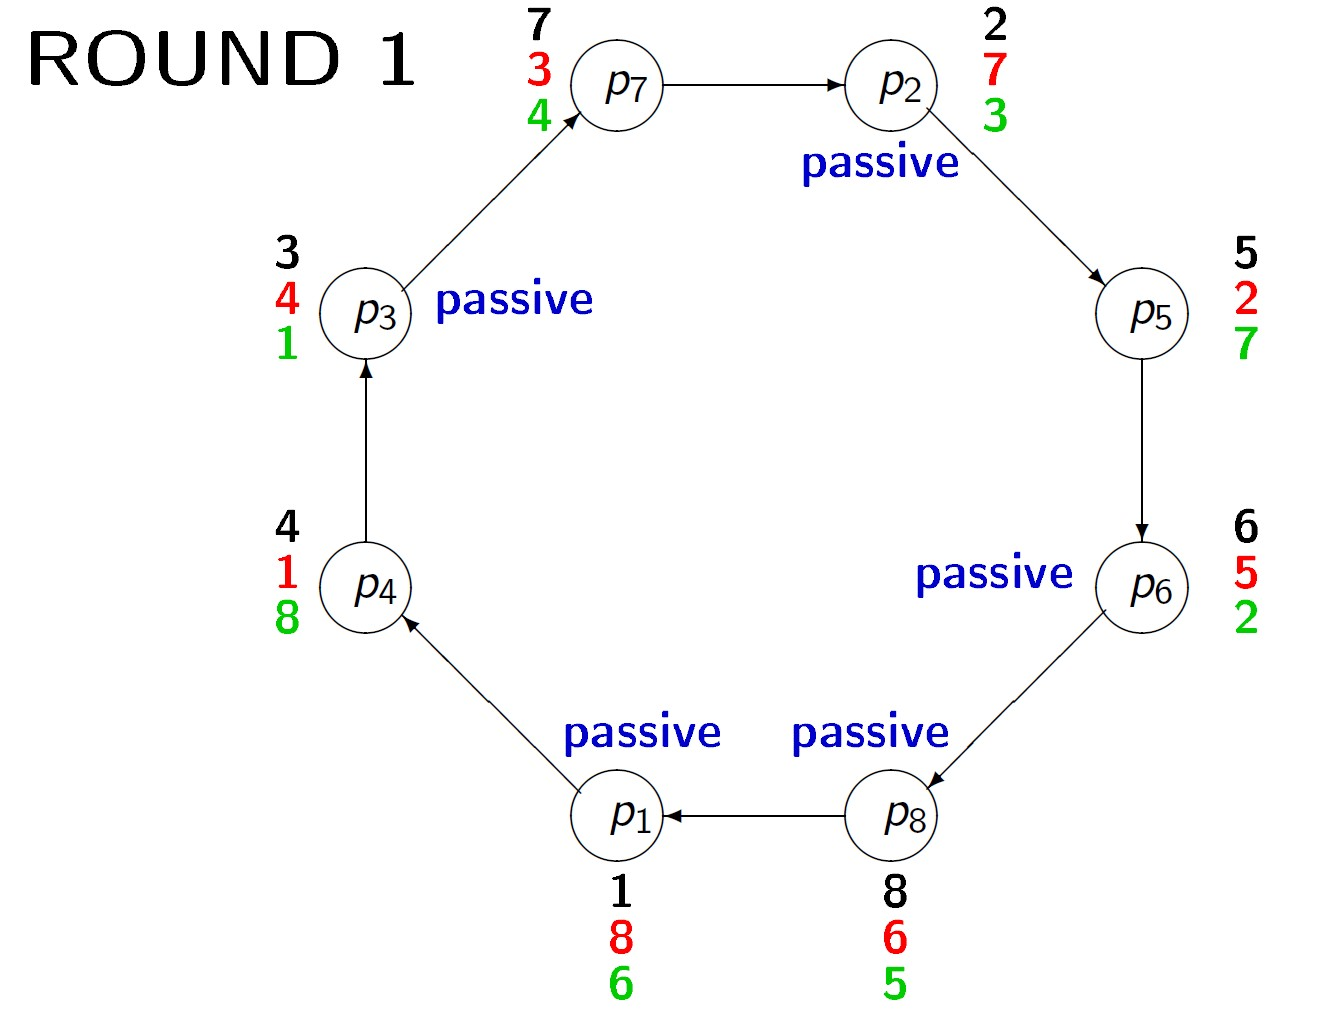
\includegraphics[scale=0.3]{figures/Screen11.jpg}
    \caption{Ring topology}
    \label{fig:Ring topology}
\end{figure}
\note{
}
\end{frame}



\begin{frame}{}
\framesubtitle{Major Results}

\begin{figure}
    \centering
    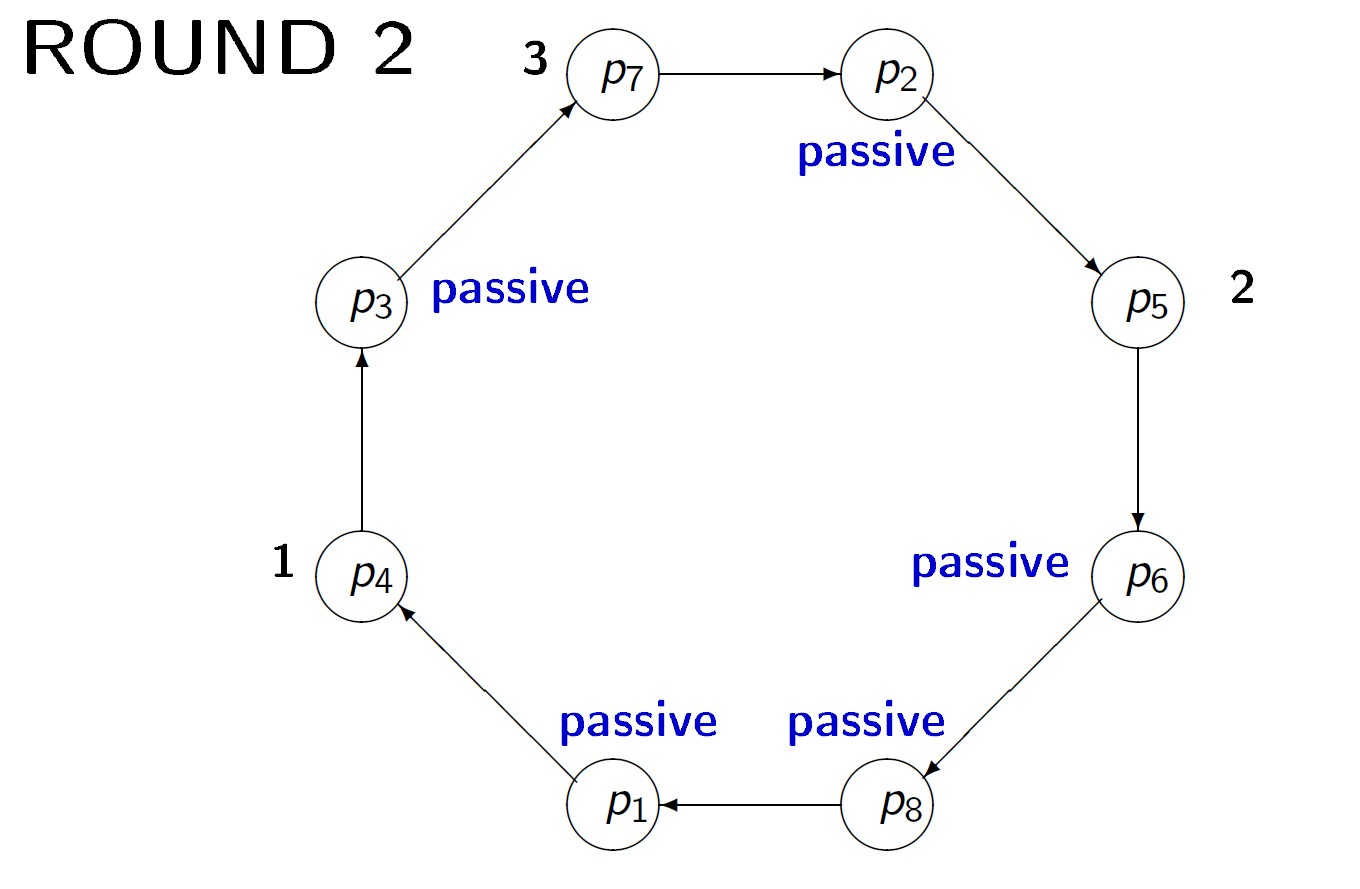
\includegraphics[scale=0.3]{figures/Screen12.jpg}
    \caption{Ring topology}
    \label{fig:Ring topology}
\end{figure}
\note{
}
\end{frame}



\begin{frame}{}
\framesubtitle{Major Results}

\begin{figure}
    \centering
    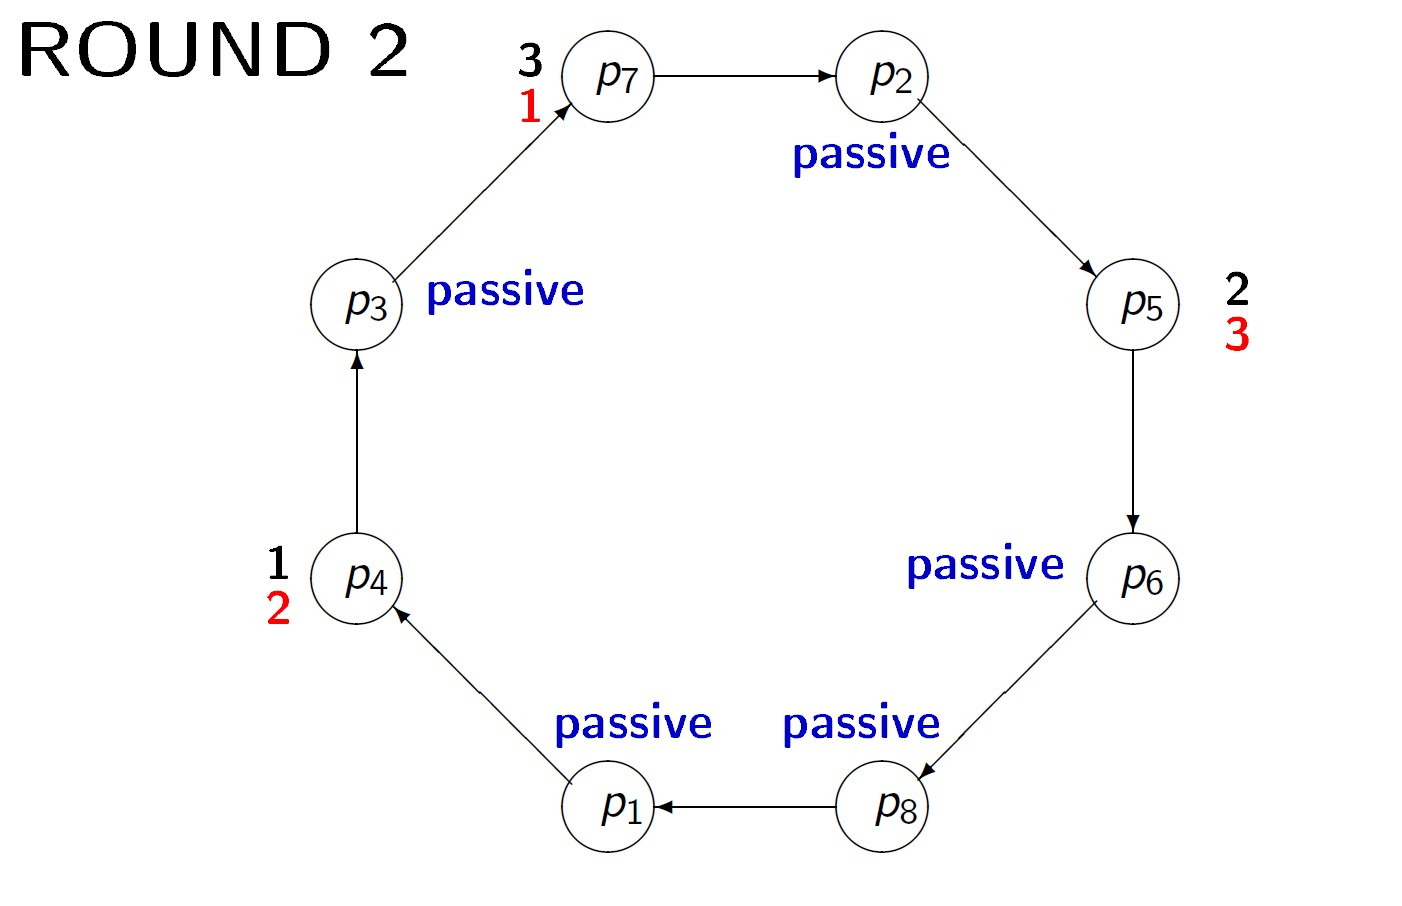
\includegraphics[scale=0.3]{figures/Screen13.jpg}
    \caption{Ring topology}
    \label{fig:Ring topology}
\end{figure}
\note{
}
\end{frame}


\begin{frame}{}
\framesubtitle{Major Results}

\begin{figure}
    \centering
    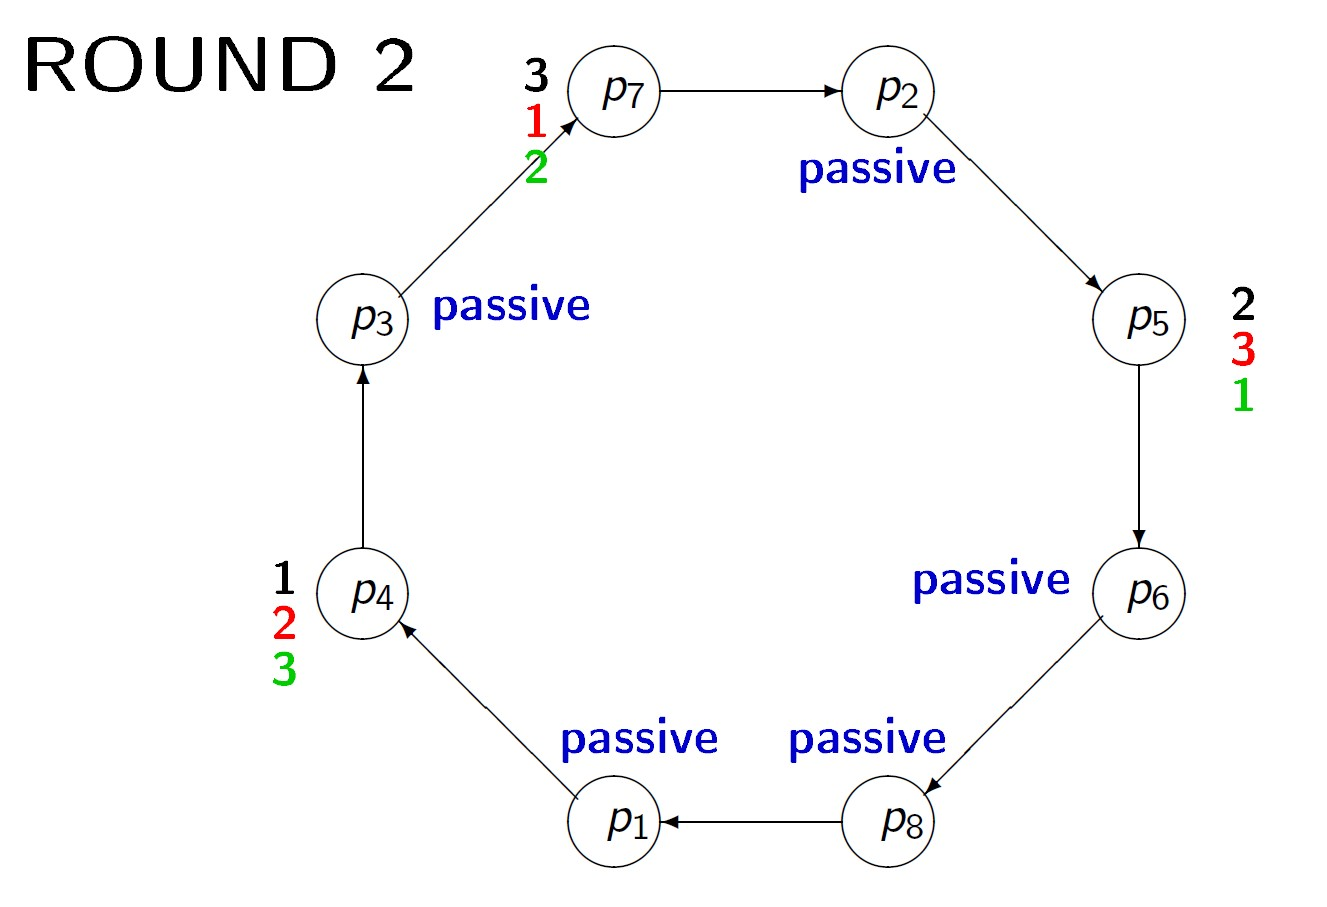
\includegraphics[scale=0.3]{figures/Screen14.jpg}
    \caption{Ring topology}
    \label{fig:Ring topology}
\end{figure}
\note{
}
\end{frame}


\begin{frame}{}
\framesubtitle{Major Results}

\begin{figure}
    \centering
    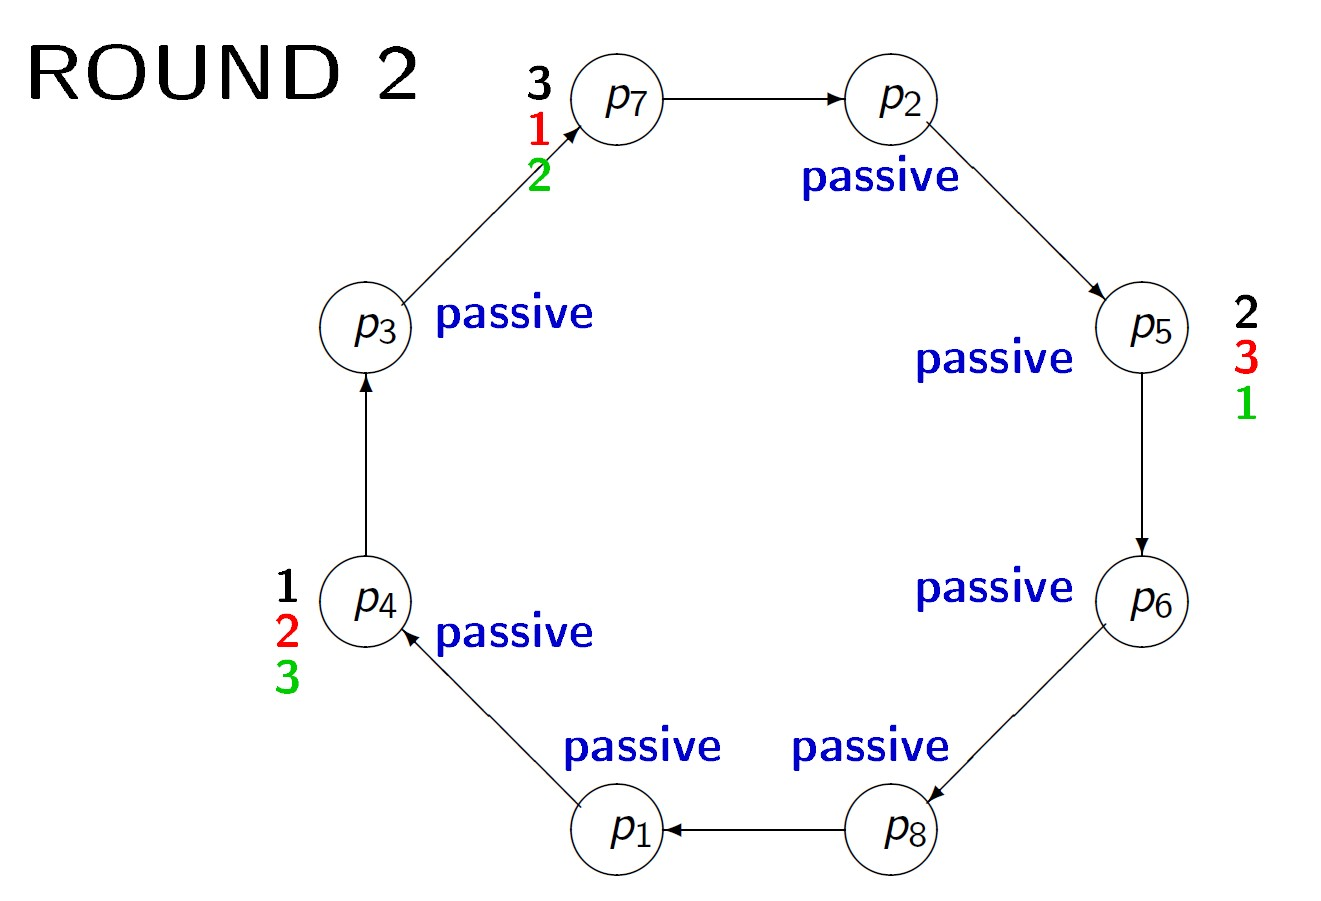
\includegraphics[scale=0.3]{figures/Screen15.jpg}
    \caption{Ring topology}
    \label{fig:Ring topology}
\end{figure}
\note{
}
\end{frame}


\begin{frame}{}
\framesubtitle{Major Results}

\begin{figure}
    \centering
    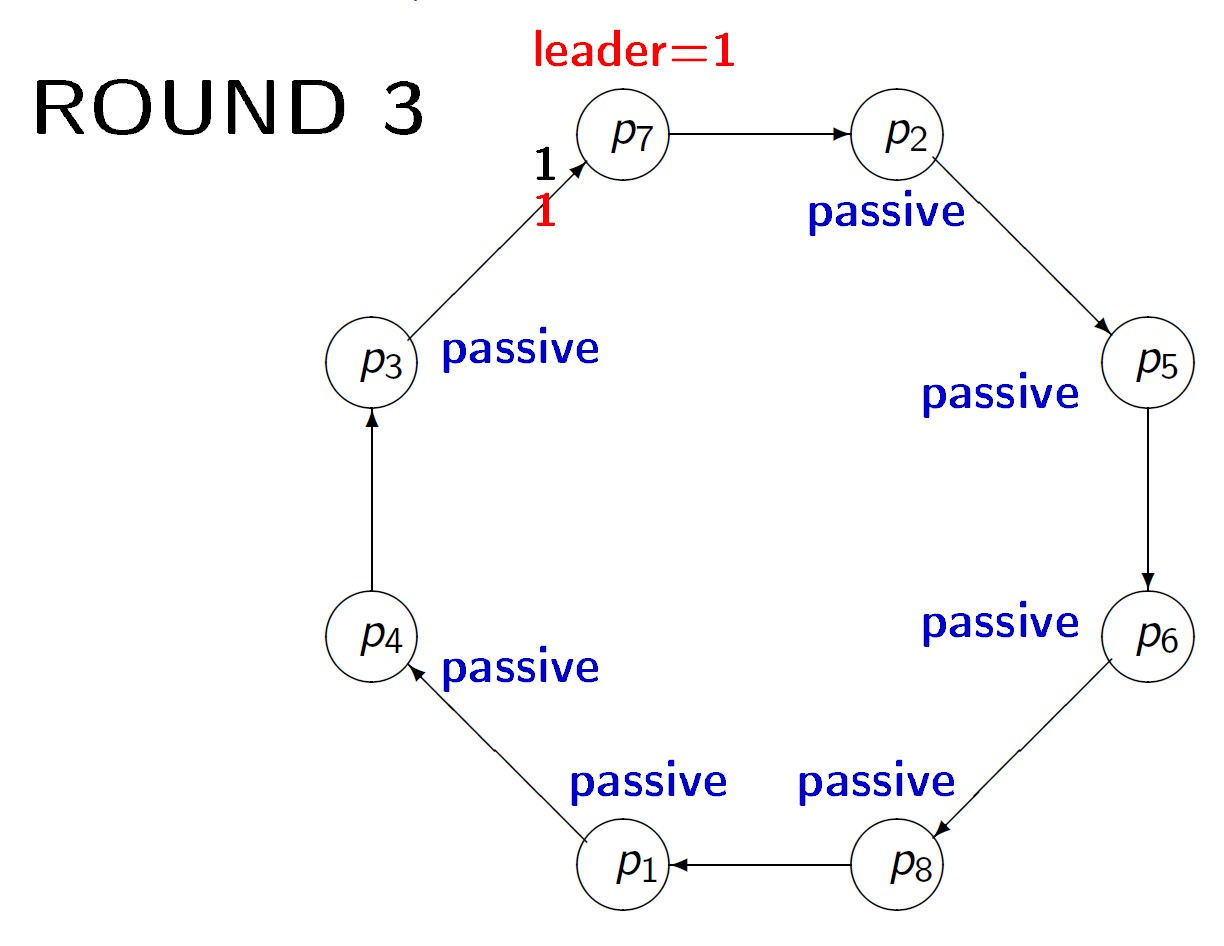
\includegraphics[scale=0.3]{figures/Screen16.jpg}
    \caption{Ring topology}
    \label{fig:Ring topology}
\end{figure}
\note{
}
\end{frame}


\begin{frame}{}
\framesubtitle{Major Results}

\begin{figure}
    \centering
    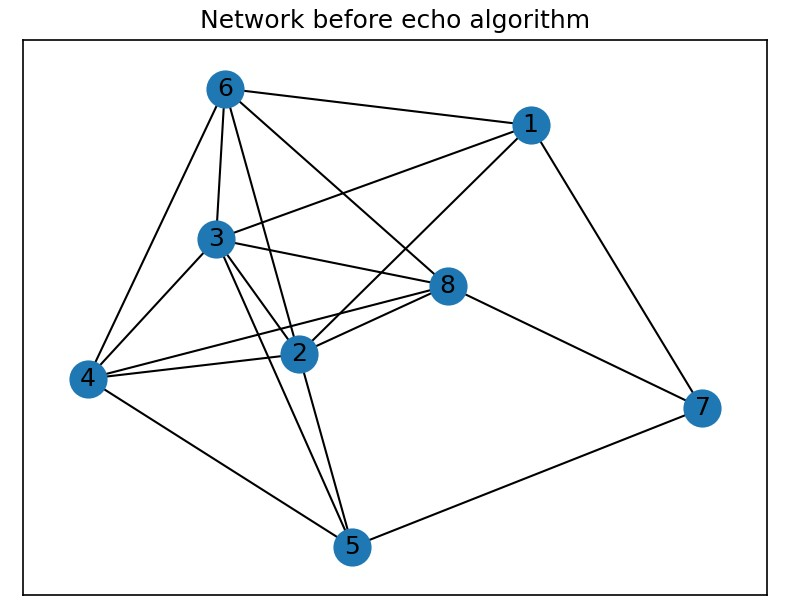
\includegraphics[scale=0.6]{figures/Screen25.jpg}
    \caption{Network Before Echo Election Algorithm}
    \label{fig:Network Before Echo Election Algorithm}
\end{figure}
\note{
}
\end{frame}


\begin{frame}{}
\framesubtitle{}

\begin{figure}
    \centering
    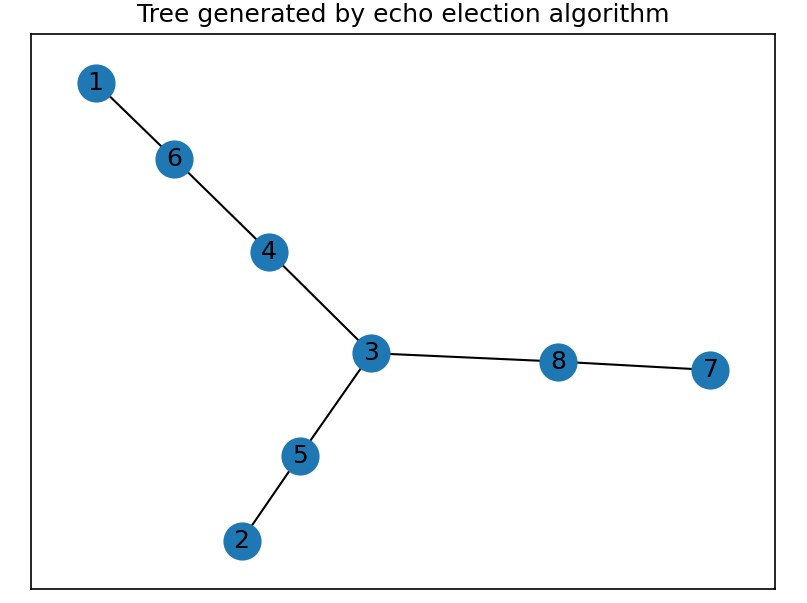
\includegraphics[scale=0.6]{figures/Screen26.jpg}
    \caption{Network After Echo Election Algorithm}
    \label{fig:Network After Echo Election Algorithm}
\end{figure}
\note{
}
\end{frame}



\begin{frame}
\frametitle{Time complexity}
The time complexity measures the number of rounds or steps required for the algorithm to complete its execution.
Eachround involves processes exchanging messages and performing local computations. 
\item The number of processes is defined as N. 
Each round in the algorithm involves each process sending and receiving messages
to and from other processes. 
Therefore, the time complexity is directly proportional to the number of messages exchanged in each round. 
\item The time complexity of the algorithm in terms of the number of messages exchanged is linear: O(E)
\end{frame}

\begin{frame}
\frametitle{Message Complexity}
The Dolev-Klawe-Rodeh Algorithm The message complexity of the algorithm can be analyzed in terms of the the number of processes (N). 
Each process needs to send a request message to every other process in the network. The message complexity of the algorithm is O(NlogN).

\end{frame}


\begin{frame}{}
\framesubtitle{Message Complexity of DKR Algorithm}

\begin{figure}
    \centering
    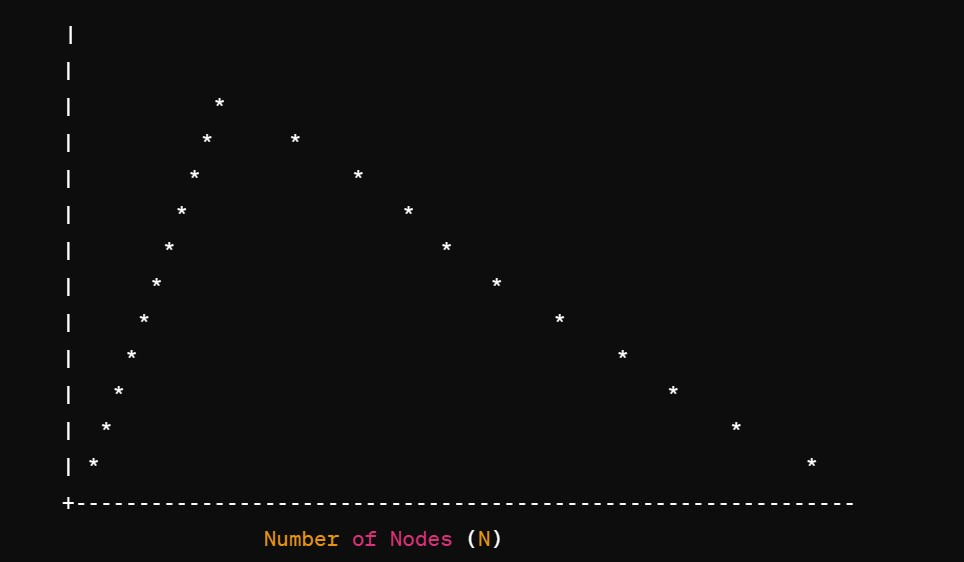
\includegraphics[scale=0.6]{figures/Screen19.jpg}
    \caption{Message Complexity of DKR Algorithm}
    \label{fig:Message Complexity}
\end{figure}
\note{
}
\end{frame}




\begin{frame}
\frametitle{Echo Algorithm with Extinction Time complexity}
Theworst case message complexity of the Echo Algorithm with Extinction is O(NE) where there are at most N waves, at most 2E message in each wave.
\end{frame}

\begin{frame}
\frametitle{Echo Algorithm with Extinction Message Complexity}
The worst case message complexity of the Echo Algorithm with Extinction is O(NE), at most 2E message in each wave.

\end{frame}


\begin{frame}{}
\framesubtitle{Message Complexity of DKR Algorithm}

\begin{figure}
    \centering
    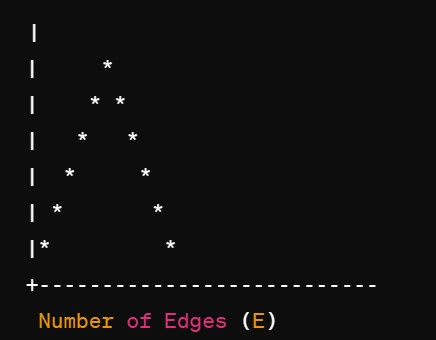
\includegraphics[scale=0.6]{figures/Screen21.jpg}
    \caption{Message Complexity of EWE Algorithm}
    \label{fig:Message Complexity}
\end{figure}
\note{
}
\end{frame}


\begin{frame}{}
\framesubtitle{Message Complexity of DKR Experiment}

\begin{figure}
    \centering
    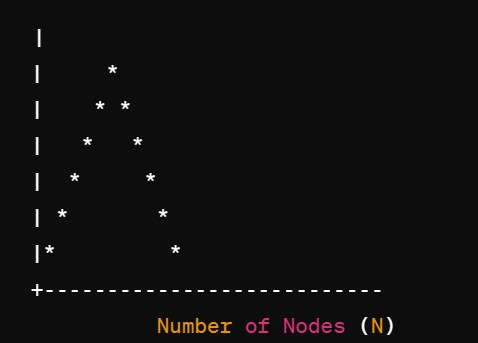
\includegraphics[scale=0.6]{figures/Screen18.jpg}
    \caption{Message Complexity of DKR Experiment}
    \label{fig:Message Complexity}
\end{figure}
\note{
}
\end{frame}


\begin{frame}{}
\framesubtitle{Message Complexity of EWE Experiment}

\begin{figure}
    \centering
    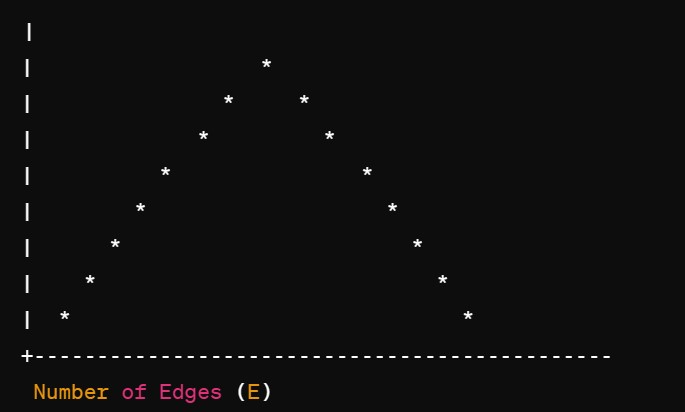
\includegraphics[scale=0.6]{figures/Screen31.jpg}
    \caption{Message Complexity of EWE Experiment}
    \label{fig:Message Complexity}
\end{figure}
\note{
}
\end{frame}




\begin{frame}
\frametitle{Result}
\framesubtitle{}

    \centering
    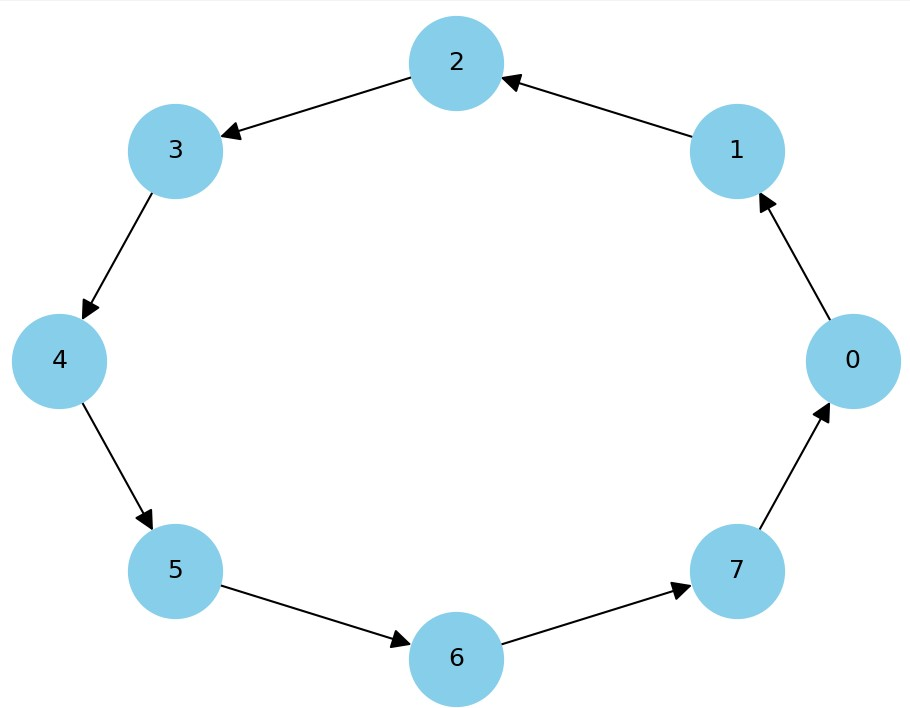
\includegraphics[scale=0.6]{figures/Screen20.jpg}
    \caption{Nodes of DKR Experiment}
    \label{fig:Message Complexity}

\end{frame}



\begin{frame}
\frametitle{Main Result of DKR Algorithm}
\begin{itemize}
\item Node 7 (ID: 7) sending alias to Node 0
 Node 0 (ID: 0) received alias 7 from Node 7
Node 0 (ID: 0) sending alias to Node 1
\item Node 1 (ID: 1) received alias 7 from Node 0
Node 1 (ID: 1) sending alias to Node 2
\item Node 2 (ID: 2) received alias 7 from Node 1
Node 2 (ID: 2) sending alias to Node 3
\item Node 3 (ID: 3) received alias 7 from Node 2
Node 3 (ID: 3) sending alias to Node 4
\item Node 4 (ID: 4) received alias 7 from Node 3
Node 4 (ID: 4) sending alias to Node 5
\item Node 5 (ID: 5) received alias 7 from Node 4
Node 5 (ID: 5) sending alias to Node 6
\item Node 6 (ID: 6) received alias 7 from Node 5
Node 6 (ID: 6) sending alias to Node 7
Node 7 (ID: 7) received alias 7 from Node 6
Node 7 is the elected leader.
Total messages sent: 44
Total messages received: 44
Leader is node 7 with alias 7
\end{itemize}
\end{frame}



\begin{frame}
\frametitle{Result}
\framesubtitle{}
The Dolev-Klawe-Rodeh (DKR) algorithm, designed for leader election in ring topologies, does not explicitly include a mechanism for dynamically handling nodes entering or leaving the network during its execution. 
Instead, it assumes a static set of nodes where each node knows the total number of nodes in the ring and can communicate with its immediate successor. 
\item Total messages sent after adding new node: 91
\item Total messages received after adding new node: 91
\item New Leader after adding node is 8 with alias 8   
\centering
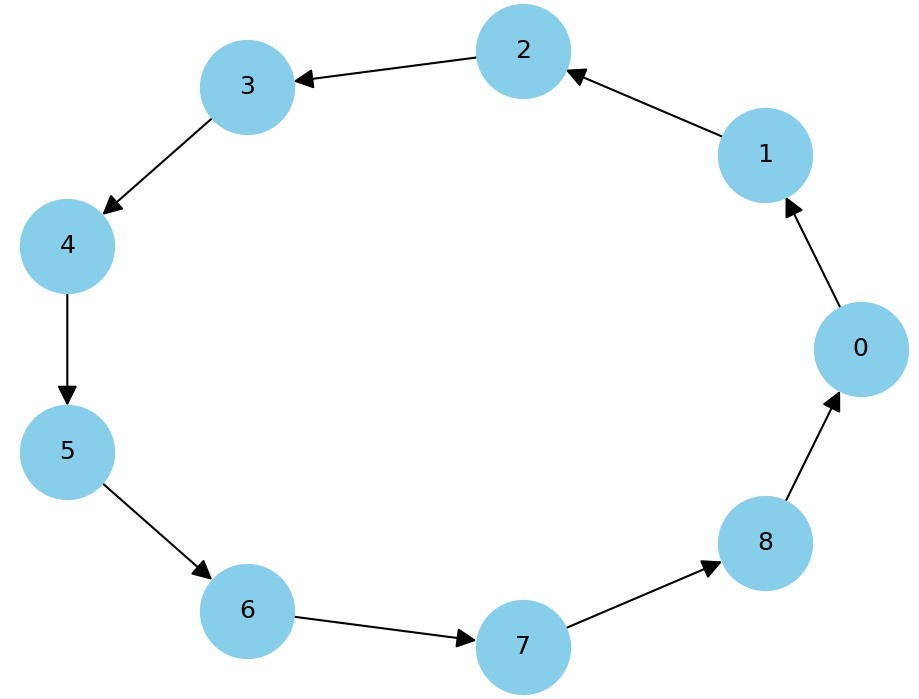
\includegraphics[scale=0.2]{figures/Screen36.jpg}
\caption{Nodes of DKR Experiment}
\label{fig:Message Complexity}

\end{frame}



\begin{frame}
\frametitle{Result}
\framesubtitle{}

    \centering
    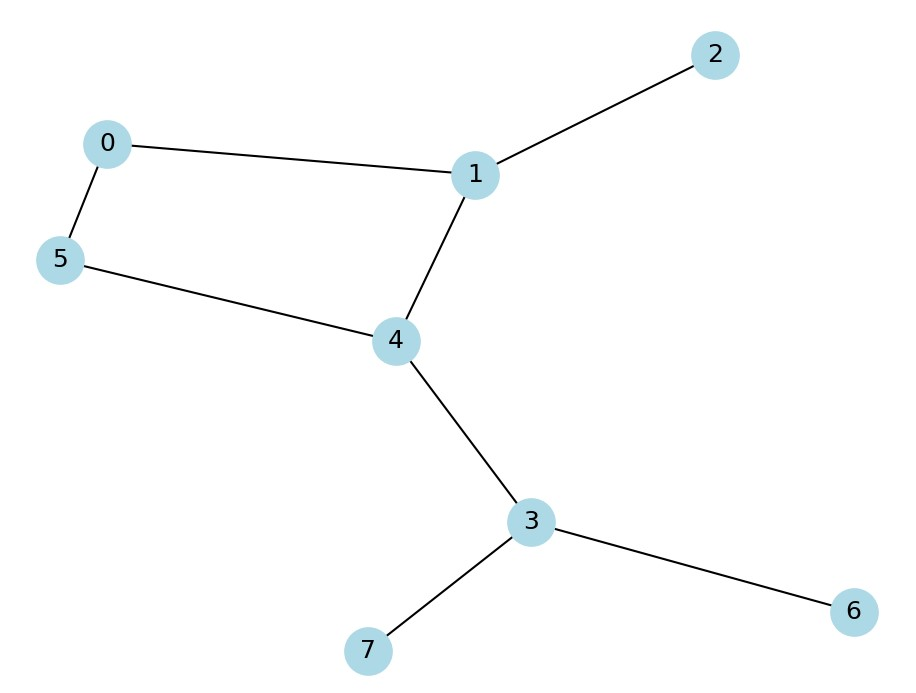
\includegraphics[scale=0.4]{figures/Screen30.jpg}
    \caption{Nodes of EWE Experiment}
    \label{fig:Message Complexity}

\end{frame}


\begin{frame}
\frametitle{Result}
\framesubtitle{}

    \centering
    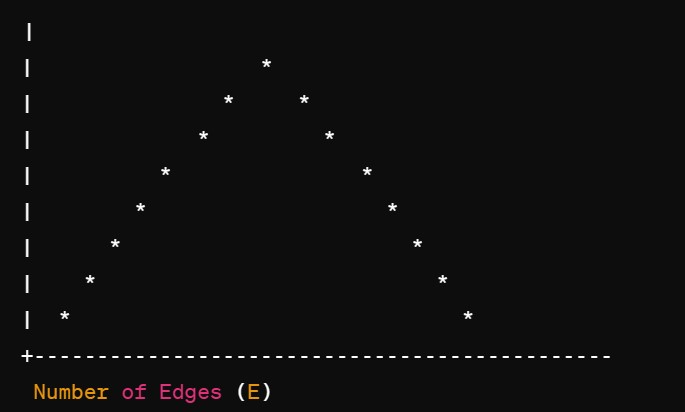
\includegraphics[scale=0.4]{figures/Screen31.jpg}
    \caption{Nodes of EWE Experiment}
    \label{fig:Message Complexity}

\end{frame}


\begin{frame}
\frametitle{Result of EWE Algorithm}
\begin{itemize}
    \centering
    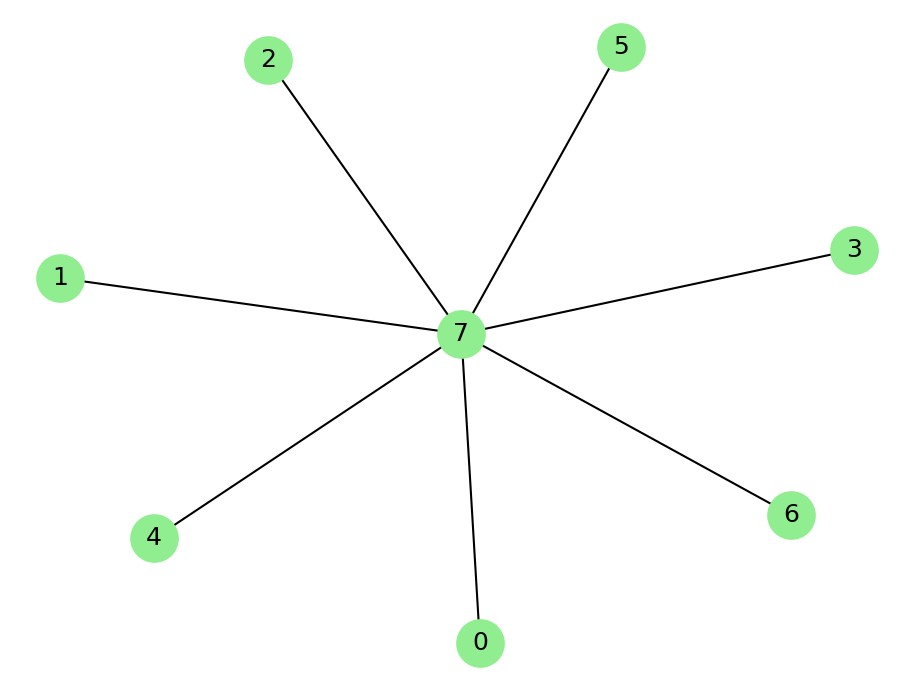
\includegraphics[scale=0.4]{figures/Screen32.jpg}
    \caption{Message Complexity of EWE Experiment}
    \label{fig:Message Complexity}   
\end{itemize}
\end{frame}



\begin{frame}
\frametitle{Conclusions}
\framesubtitle{}
\begin{itemize}
\item The DKR algorithm is effective in ring-based networks with potentially large IDs and where the communication delay between nodes is uniform or predictable. It is more message-efficient compared to simpler algorithms. 
\item The Echo with Extinction algorithm offers an average-case complexity of O(N) making it an attractive option for scenarios where minimizing message passing is a priority. 
The extinction mechanism prevents nodes from perpetually echoing messages in isolated segments, promoting convergence towards a leader even amidst network disruptions.


\end{itemize}

\end{frame}


\begin{frame}{References}

Wan Fokkink, Distributed Algorithms An Intuitive Approach, The MIT Press Cambridge, Massachusetts London, England, 2013
\item Gerard Tel, Introduction to Distributed Algorithms, CAMBRIDGE UNIVERSITY PRESS, 2001
\item Leslie Lamport, K. Mani Chandy: Distributed Snapshots: Determining Global States of a Distributed System. In: ACM Transactions on Computer Systems 3. Nr. 1, Februar 1985.
\item Michel Raynal, Distributed Algorithms for Message-Passing Systems, Springer, 2013
\bibliographystyle{IEEEtran}
\bibliography{refs}
\end{frame}



\end{document}